% CS6101 final presentation. Compile on Overleaf (pdfLaTeX) in the same project as main.tex,
% so the figures/ folder is shared. About 12 minutes, 10 slides (limit: 10).
\documentclass[aspectratio=169,11pt]{beamer}

\usepackage[T1]{fontenc}
\usepackage{lmodern}
\usepackage{booktabs}
\usepackage{graphicx}

% ---------- look: plain, one accent colour matching the figures (Okabe-Ito blue) ----------
\definecolor{accent}{HTML}{0072B2}
\definecolor{ink}{HTML}{222222}
\definecolor{muted}{HTML}{666666}
\setbeamercolor{normal text}{fg=ink}
\setbeamercolor{frametitle}{fg=accent}
\setbeamercolor{title}{fg=accent}
\setbeamercolor{structure}{fg=accent}
\setbeamercolor{alerted text}{fg=accent}
\setbeamerfont{frametitle}{series=\bfseries,size=\Large}
\setbeamertemplate{navigation symbols}{}
\setbeamertemplate{itemize items}{\textbullet}
\setbeamertemplate{footline}{\hfill\textcolor{muted}{\scriptsize\insertframenumber\,/\,\inserttotalframenumber}\hspace{1em}\vspace{0.6em}}
\setlength{\parskip}{0.4em}

\newcommand{\takeaway}[1]{\vfill\begin{center}\textcolor{accent}{\textbf{#1}}\end{center}}

\title{Disclosure Without Inference}
\subtitle{LLM Agents Anchor on Disclosed Trade Data When Bargaining}
\author{Joey Poh}
\institute{CS6101 Rational Approaches to Cooperative Intelligence\\National University of Singapore}
\date{November 2026}

\begin{document}

% ======================================================================
\begin{frame}[plain]
  \titlepage
\end{frame}

% ======================================================================
\begin{frame}{Motivation and research question}
  \begin{itemize}
    \item AI agents are starting to negotiate trades for people, and one side may field a far more capable model. Which protocols still protect the weaker side? \textcolor{muted}{(AGI Institutions)}
    \item One proposal: an \alert{information floor}, giving the weaker side information it cannot infer itself. When US corporate bond trades were published (TRACE), investors' trading costs fell \textcolor{muted}{(Goldstein et al., 2007)}.
  \end{itemize}
  \vspace{0.3em}
  \begin{enumerate}
    \item Does disclosing other dealers' trade data \alert{improve} an LLM client's outcome when it bargains with a dealer?
    \item Does the client use the disclosure \alert{as a Bayesian would}, or merely \alert{anchor} on its numbers?
  \end{enumerate}
  \vspace{0.3em}
  \small Setting: a client buys \$10mm of an off-the-run 10-year US Treasury note from a single dealer whose cost is private.
  Off-the-run trades are reported to FINRA but not published: the band models publishing them.
\end{frame}

% ======================================================================
\begin{frame}{The game}
  \centering
  \vspace{-0.6em}
  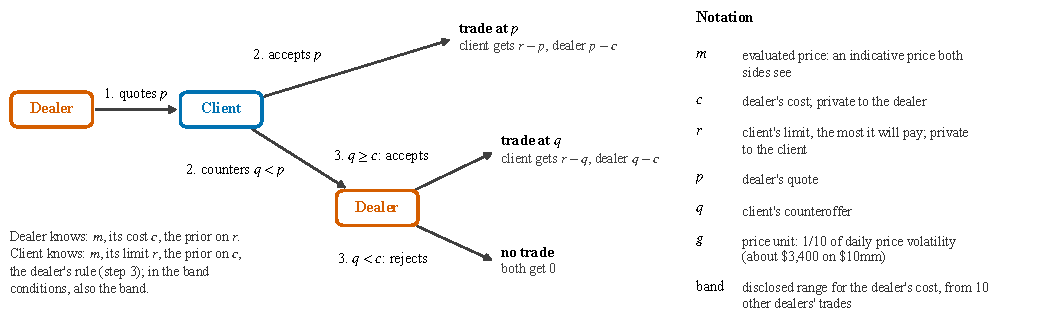
\includegraphics[height=3.0cm]{figures/fig1_setup.pdf}\\[0.2em]
  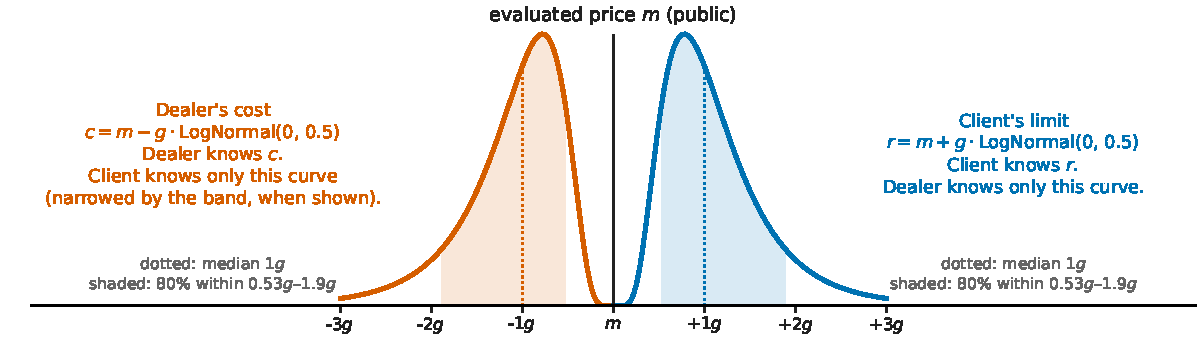
\includegraphics[height=3.0cm]{figures/fig_priors.pdf}

  \vspace{0.2em}
  \raggedright\footnotesize
  Prices are measured in $g$, one tenth of the note's daily price volatility (about \$3,400 on \$10mm).
  The client's \alert{briefing} states the cost distribution as gaps and, for convenience, as prices: a typical dealer cost of $m - 1g$; 80\% of costs between $m - 1.9g$ and $m - 0.53g$.
  Outcome: the client's \alert{share of the surplus}, $(r - \text{price})/(r - c)$, or 0 if no trade.
\end{frame}

% ======================================================================
\begin{frame}{The band, the Bayesian benchmark and the design}
  \begin{columns}[T]
    \begin{column}{0.5\textwidth}
      \small
      In some conditions the client also reads:
      \begin{quote}\footnotesize
        ``Reported purchases by other dealers of similar off-the-run notes yesterday (10 trades) \ldots\ imply a typical dealer cost of \textit{avg}. \ldots\ this dealer's own cost is within [\textit{low}, \textit{high}] about two times in three.''
      \end{quote}
      \begin{itemize}
        \item A noisy but accurate reading of the dealer's cost.
        \item \textbf{Bayesian client}: combines the band with its prior and bids optimally. Against the same fixed dealer, the band raises its share from \alert{62\% to 73\%}.
      \end{itemize}
    \end{column}
    \begin{column}{0.47\textwidth}
      \small
      \textbf{2 $\times$ 2 conditions}\\[0.3em]
      \begin{tabular}{@{}lcc@{}}
        \toprule
        & No band & Band \\
        \midrule
        No belief elicitation & \checkmark & \checkmark \\
        Belief elicitation & \checkmark & \checkmark \\
        \bottomrule
      \end{tabular}
      \begin{itemize}
        \item Elicitation, before and after the quote: {\footnotesize ``For each price below, give your probability \ldots\ that the dealer's cost is below that price.''} Nine fixed prices, $0.25g$ to $3g$ below $m$.
        \item Client: Ornith-1.5-35B, temperature 0.5, reasoning off; chosen by a pilot fixed in advance.
        \item 50 scenarios $\times$ 2 runs; 20 held-out scenarios.
      \end{itemize}
    \end{column}
  \end{columns}
  \takeaway{The most a client that uses the band perfectly can gain: 11\% of the surplus}
\end{frame}

% ======================================================================
\begin{frame}{Result 1: the band did not help}
  \begin{columns}[c]
    \begin{column}{0.52\textwidth}
      \centering
      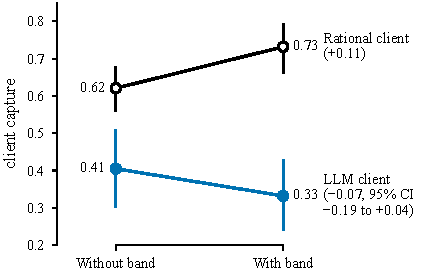
\includegraphics[width=\textwidth]{figures/fig2_results.pdf}
    \end{column}
    \begin{column}{0.45\textwidth}
      \begin{itemize}
        \item Without belief elicitation: 41\% $\rightarrow$ 33\% of the surplus.
        \item Difference $-7.3$ points, 95\% CI [$-19.0$, $3.8$]: \alert{main test not supported}.
        \item Paired test: the LLM gained 18 points less than the Bayesian client (95\% CI [5, 32], $p \approx 0.008$).
      \end{itemize}
    \end{column}
  \end{columns}
\end{frame}

% ======================================================================
\begin{frame}{Result 2: the client bids the numbers it is given}
  \begin{columns}[c]
    \begin{column}{0.5\textwidth}
      \centering
      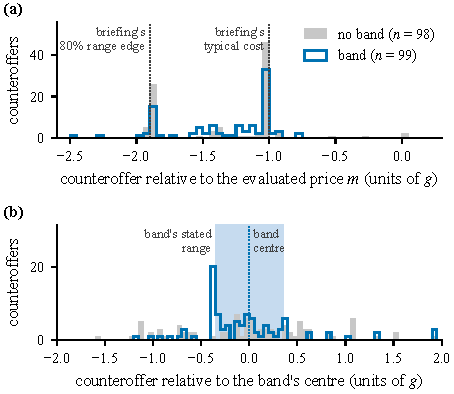
\includegraphics[width=\textwidth]{figures/fig3_counters.pdf}
    \end{column}
    \begin{column}{0.48\textwidth}
      \begin{itemize}\footnotesize
        \item Every briefing says: {\scriptsize ``the median gap is $1g$, and 80\% of dealers' gaps lie between $0.53g$ and $1.9g$. In prices, a typical dealer's cost is about \alert{[$m - 1g$]}, and 80\% of dealers' costs lie between \alert{[$m - 1.9g$]} and [$m - 0.53g$].''}
        \item Without the band: 77 of 98 bids sit on the two highlighted prices.
        \item The client reacted to the band: bids moved $0.16g$ closer to its typical cost, but 26\% sat on the band's \alert{lowest price}, where the cost is below only $\sim$16\% of the time, so \alert{77\% were rejected}.
        \item Belief elicitation's own prices became anchors too.
      \end{itemize}
    \end{column}
  \end{columns}
  \takeaway{Anchoring, not inference}
\end{frame}

% ======================================================================
\begin{frame}{Result 3: it weighs evidence the wrong way round}
  \begin{columns}[c]
    \begin{column}{0.52\textwidth}
      \centering
      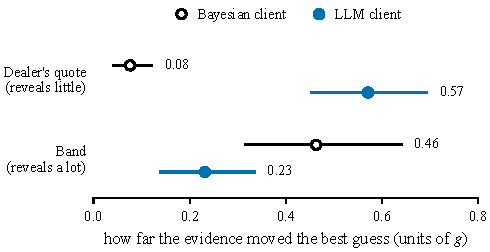
\includegraphics[width=\textwidth]{figures/fig4_evidence.pdf}
    \end{column}
    \begin{column}{0.45\textwidth}
      \begin{itemize}\small
        \item The \textbf{quote} reveals almost nothing: the dealer quotes the same price whatever its cost.
        \item Yet it moved the LLM's best guess \alert{$0.57g$}, against $0.08g$ for a Bayesian.
        \item The \textbf{band} reveals a lot, yet moved it only \alert{$0.23g$}, against $0.46g$.
        \item Its bids barely followed its own stated beliefs.
      \end{itemize}
    \end{column}
  \end{columns}
\end{frame}

% ======================================================================
\begin{frame}{Confirmation on unseen scenarios}
  \begin{columns}[c]
    \begin{column}{0.48\textwidth}
      \centering
      
\includegraphics[width=0.95\textwidth]{figures/fig5_heldout.pdf}
    \end{column}
    \begin{column}{0.5\textwidth}
      \begin{itemize}\small
        \item 20 scenarios never used in development; analysis code unchanged.
        \item (a) Again no reliable effect on the client's share.
        \item (b) Again bids move towards the band's centre: \alert{anchoring replicates}.
        \item (c) Beliefs again lag the Bayesian's, and on these scenarios do not move at all.
      \end{itemize}
    \end{column}
  \end{columns}
\end{frame}

% ======================================================================
\begin{frame}{Limitations}
  \begin{itemize}
    \item \textbf{Simplified market}: one dealer, one counteroffer, walking away worth nothing.
    \item \textbf{Fixed dealer}: it neither adapts to nor exploits the client, and its quote reveals little.
    \item \textbf{Synthetic values}: only the price scale is calibrated to market data.
    \item \textbf{One model}, reasoning off, one prompt.
    \item The briefing states the cost distribution as \textbf{concrete prices}, which themselves became anchors.
  \end{itemize}
  \vspace{0.5em}
  \textbf{Next}: reasoning on; other models and sizes; the briefing without price levels.
\end{frame}

% ======================================================================
\begin{frame}{Takeaways}
  \begin{enumerate}
    \item \alert{Disclosure cannot substitute for inference the agent does not perform.} The LLM noticed the band but bid its numbers.
    \item \alert{Presentation matters as much as disclosure.} An anchoring agent bids whatever number it is shown.
    \item \alert{Asking about beliefs is not neutral.} The question's own prices became bids.
    \item Information floors alone may not protect weaker agents: marketplaces may also need \alert{minimum capability standards}, which games with a Bayesian benchmark could help test.
  \end{enumerate}
  \vfill
  \begin{center}\textcolor{accent}{\textbf{Thank you. Questions?}}\end{center}
  \vspace{0.3em}
  \raggedright\tiny\textcolor{muted}{
  AGI Institutions Wiki (2026). Agent negotiation \& bargaining. \quad
  Goldstein, Hotchkiss \& Sirri (2007). \textit{Review of Financial Studies} 20(2). \quad
  Myerson \& Satterthwaite (1983). \textit{Journal of Economic Theory} 29(2). \quad
  Tversky \& Kahneman (1974). \textit{Science} 185(4157).}
\end{frame}

\end{document}
